\documentclass[11pt,letterpaper]{article}
\usepackage[utf8]{inputenc}
\usepackage[T1]{fontenc}
\usepackage[spanish]{babel}
\usepackage{amsmath}
\usepackage{amsfonts}
\usepackage{amssymb}
\usepackage{graphicx}
\usepackage{lmodern}
\usepackage{xspace}
\usepackage{multicol}
\usepackage{hyperref}
\usepackage{float}
\usepackage{hyperref}
\usepackage{color}
\usepackage{framed}



\usepackage[left=2cm,right=2cm,top=2cm,bottom=2cm]{geometry}

\newcommand{\X}{\mathbb{X}}
\newcommand{\x}{\mathbf{x}}
\newcommand{\Y}{\mathbf{Y}}
\newcommand{\y}{\mathbf{y}}
\newcommand{\xbarn}{\bar{x}_n}
\newcommand{\ybarn}{\bar{y}_n}
\newcommand{\paren}[1]{\left( #1 \right)}
\newcommand{\llaves}[1]{\left\lbrace #1 \right\rbrace}
\newcommand{\barra}{\,\vert\,}
\newcommand{\mP}{\mathbb{P}}
\newcommand{\mE}{\mathbb{E}}
\newcommand{\mR}{\mathbb{R}}
\newcommand{\mJ}{\mathbf{J}}
\newcommand{\mX}{\mathbf{X}}
\newcommand{\mS}{\mathbf{S}}
\newcommand{\mA}{\mathbf{A}}
\newcommand{\unos}{\boldsymbol{1}}
\newcommand{\xbarnv}{\bar{\mathbf{x}}_n}
\newcommand{\abs}[1]{\left\vert #1 \right\vert}
\newcommand{\muv}{\boldsymbol{\mu}}
\newcommand{\mcov}{\boldsymbol{\Sigma}}
\newcommand{\vbet}{\boldsymbol{\beta}}
\newcommand{\veps}{\boldsymbol{\epsilon}}
\newcommand{\mcC}{\mathcal{C}}
\newcommand{\mcR}{\mathcal{R}}
\newcommand{\mcN}{\mathcal{N}}

\newcommand{\ceros}{\boldsymbol{0}}
\newcommand{\mH}{\mathbf{H}}
\newcommand{\ve}{\mathbf{e}}
\newcommand{\avec}{\mathbf{a}}
\newcommand{\res}{\textbf{RESPUESTA}\\}

\newcommand{\defi}[3]{\textbf{Definición:#3}}
\newcommand{\fin}{$\blacksquare.$}
\newcommand{\finf}{\blacksquare.}
\newcommand{\tr}{\text{tr}}
\newcommand*{\temp}{\multicolumn{1}{r|}{}}

\newcommand{\grstep}[2][\relax]{%
   \ensuremath{\mathrel{
       {\mathop{\longrightarrow}\limits^{#2\mathstrut}_{
                                     \begin{subarray}{l} #1 \end{subarray}}}}}}
\newcommand{\swap}{\leftrightarrow}

\newcommand{\gen}{\text{gen}}
\newtheorem{thmt}{Teorema:}
\newtheorem{thmd}{Definición:}
\newtheorem{thml}{Lema:}

\begin{document}
\begin{table}[ht]
\centering
\begin{tabular}{c}
\textbf{Control de la tasa de falsos descubrimientos: un enfoque práctico y potente para pruebas múltiples.}\\
\emph{Yoav Benjamini; Yosef Hochberg}\\
\emph{Traducción del artículo (\textit{no oficial})}
\end{tabular}
\end{table}

\section*{Resumen}
El enfoque común del problema de la multiplicidad exige controlar la tasa de error familiar (FWER). Sin embargo, este enfoque tiene fallas y señalamos algunas. Se presenta un enfoque diferente a los problemas de pruebas de significancia múltiple. Requiere controlar la proporción esperada de hipótesis falsamente rechazadas: la tasa de falsos descubrimientos. Esta tasa de error es equivalente a la FWER cuando todas las hipótesis son verdaderas pero es menor en caso contrario. Por lo tanto, en los problemas en los que se desea el control de la tasa de descubrimiento falso en lugar del de FWER, existe la posibilidad de una ganancia de potencia. Se ha demostrado que un procedimiento secuencial simple de Bonferronitype controla la tasa de descubrimiento falso para las estadísticas de prueba independientes, y un estudio de simulación muestra que la ganancia de potencia es sustancial. El uso del nuevo procedimiento y la idoneidad del criterio se ilustran con ejemplos.

\section{INTRODUCIÓN}
Cuando se realizan inferencias múltiples, los investigadores tienden a seleccionar las significativas (estadísticamente) para enfatizar, discutir y apoyar las conclusiones. Un uso descuidado de procedimientos de inferencia única da como resultado una tasa de falsos positivos (significancia) mucho mayor. Para controlar este efecto de multiplicidad (selección), los procedimientos clásicos de comparación múltiple (MCP) tienen como objetivo controlar la probabilidad de cometer cualquier error de tipo 1 en familias de comparaciones bajo consideración simultánea. El control de esta tasa de error familiar (FWER) generalmente se requiere en un sentido fuerte, es decir, bajo todas las configuraciones de hipótesis verdaderas y falsas probadas (ver, por ejemplo, Hochberg y Temhane (1987)).\\

Aunque los MCP se han utilizado desde principios de 1950, y a pesar de la defensa de su uso, (por ejemplo, siendo obligatorio para algunas revistas, así como en algunas instituciones como la Administración de Alimentos y Medicamentos de los EE. UU.), los investigadores aún no han adoptado ampliamente estos procedimientos. En la investigación médica, por ejemplo, Godfrey (1985), Pocock et al. (1987) y Smith et al (1987) examinaron muestras de informes de estudios comparativos de las principales revistas médicas. Descubrieron que los investigadores pasan por alto varios tipos de multiplicidad y, como resultado, los informes tienden a exagerar las diferencias de tratamiento (Pocock et al., 1987).\\
Algunas de las dificultades del MCP clásico que provocan su subutilización en la investigación aplicada son las siguientes.
\begin{itemize}
\item[(a)] Gran parte de la metodología de FWER que controla MCP se refiere a comparaciones de múltiples tratamientos y familias cuyas estadísticas de prueba son multivariadas normales (o t). En la práctica, muchos de los problemas encontrados no son del tipo de tratamientos múltiples y las estadísticas de las pruebas no son normales multivariadas. De hecho, las familias a menudo se combinan con estadísticas de diferentes tipos.

\item[b)] Los procedimientos clásicos que controlan el FWER en sentido estricto, en niveles convencionales en problemas de comparación única, tienden a tener sustancialmente menos poder que el procedimiento por comparación de los mismos niveles.

\item[c)] A menudo, el control del FWER no es del todo necesario. El control del FWER es importante cuando es probable que una conclusión de las diversas inferencias individuales sea errónea cuando al menos una de ellas lo es. Este puede ser el caso, por ejemplo, cuando varios tratamientos nuevos compiten contra un estándar y se elige un único tratamiento del conjunto de tratamientos que se declaran significativamente mejores que el estándar. Sin embargo, un grupo de tratamiento y un grupo de control a menudo se comparan probando varios aspectos del efecto (diferentes puntos finales en la terminología de los ensayos clínicos). La conclusión general de que el tratamiento es superior no tiene por qué ser errónea incluso si algunas de las hipótesis nulas se rechazan falsamente.
\end{itemize}

La primera dificultad ha sido abordada parcialmente por la reciente línea de investigación que avanza en procedimientos tipo Bonferroni, que utilizan los valores p individuales observados, sin dejar de ser fieles al control FWER: Simes (1986), Hommel (1988), Hochberg (1988) y Rom (1990). Las otras dos dificultades aún presentan un problema grave. Esta es probablemente la razón por la que algunos todavía recomiendan un enfoque de tasa de error por comparación (PCER), que equivale a ignorar por completo el problema de la multiplicidad (por ejemplo, Saville (1990)).\\
En este trabajo proponemos un nuevo punto de vista sobre el problema de la multiplicidad. En muchos problemas de multiplicidad debe tenerse en cuenta el número de rechazos erróneos y no solo la cuestión de si se cometió algún error. Sin embargo, al mismo tiempo, la gravedad de la pérdida incurrida por rechazos erróneos está inversamente relacionada con el número de hipótesis rechazadas. Desde este punto de vista, una tasa de error deseable a controlar puede ser la proporción esperada de errores entre las hipótesis rechazadas, que denominamos tasa de descubrimiento falso (FDR). Este criterio integra la preocupación de Spjøtvoll (1972) sobre el número de errores cometidos en problemas de comparación múltiple, con la preocupación de Soric (1989) sobre la probabilidad de un falso rechazo dado un rechazo. Usamos el término FDR después de Soric (1989), quien identificó una hipótesis rechazada con un ''descubrimiento estadístico''.\\
Después de algunos preliminares, presentamos en la Sección 2.1 una definición formal del FDR. Se dan dos consecuencias inmediatas pero importantes de controlar esta tasa de error: implica un control débil de FWER y admite procedimientos más potentes. En la Sección 2.2 presentamos algunos ejemplos donde es deseable el control del FDR. En la Sección 3 presentamos un procedimiento de control FDR simple tipo Bonferroni y el resto de la sección está dedicado a una discusión y demostración de sus propiedades. La sección 4 presenta un estudio de simulación de la potencia del procedimiento.

\section{Tasa de descubrimiento Falso (False Discovery Rate)}
Considere el problema de probar simultáneamente $m$ hipótesis (nulas), de las cuales $m_0$ son verdaderas. $R$ es el número de hipótesis rechazadas.

\begin{figure}[H]
\centering
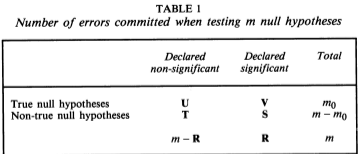
\includegraphics[scale=.8]{tabla_1.png}
\end{figure}

La Tabla 1 resume la situación en forma tradicional. Se supone que las hipótesis $m$ específicas se conocen de antemano. $R$ es una variable aleatoria observable; $U, V, S $ y $T$ son variables aleatorias no observables. Si cada hipótesis nula individual se prueba por separado en el nivel $\alpha$, entonces $R=R (\alpha)$ aumenta en $\alpha$. Usamos las letras minúsculas equivalentes para sus valores realizados.

En términos de estas variables aleatorias, el PCER es $E(V/m)$ y el FWER es $P(V\geq 1)$. Probar individualmente cada hipótesis en el nivel $\alpha$ garantiza que $\mE(V / m) <\alpha$. Probar individualmente cada hipótesis en el nivel $\alpha/m$ garantiza que $P (V\geq 1) <\alpha$.

\subsection{Definición de tasa de descubrimiento falso (False Discovery Rate)} 
La proporción de errores cometidos al rechazar falsamente hipótesis nulas se puede ver a través de la variable aleatoria $Q=V/(V + S)$, la proporción de hipótesis nulas rechazadas que se rechazan erróneamente. Naturalmente, definimos $Q = 0$ cuando $V + S = 0$, ya que no se puede cometer ningún error de falso rechazo. $Q$ es una variable aleatoria no observada (desconocida), ya que no conocemos $v$ o $s$, y por lo tanto $q = v / (v + s)$, incluso después de la experimentación y el análisis de datos. Definimos el FDR $Q_e$ como la experanza de $Q$,
$$Q_e = E (Q) = E\{V / (V + S)\} = E (V / R).$$
Dos propiedades de esta tasa de error se muestran fácilmente, pero son muy importantes.
\begin{itemize}
\item[(a)] Si todas las hipótesis nulas son verdaderas, el FDR es equivalente al FWER: en este caso $s = 0$ y $v = r$, entonces si $y = 0$ entonces $Q = 0$, y si $v> 0$ entonces $Q = 1$, lo que conlleva a $P (V> 1) = E (Q) = Q_e$. Por lo tanto, el control del FDR implica el control del FWER en el sentido débil.
\item[b)] Cuando $m_0<m$, el FDR es menor o igual que el FWER: en este caso, si $v>0$ entonces $v/r<1$, lo que lleva a que $X_{(V>1)}>Q$. Tomando expectativas en ambos lados obtenemos $P(V> 1)> Q_e$, y los dos pueden ser bastante diferentes. Como resultado, cualquier procedimiento que controle el FWER también controla el FDR. Sin embargo, si un procedimiento controla únicamente el FDR, puede ser menos estricto y se puede esperar una ganancia de potencia. En particular, cuanto mayor es el número de hipótesis nulas no verdaderas, mayor tiende a ser $S$, y también lo es la diferencia entre las tasas de error. Como resultado, el potencial de aumento de potencia es mayor cuando la mayoría de las hipótesis son falsas.
\end{itemize}

\subsection{Ejemplos}
Los siguientes ejemplos muestran la relevancia del control FDR en algunas situaciones típicas. Además, indican la conveniencia de un gran número de rechazos (descubrimientos). Ambos aspectos se abordan mediante el procedimiento que se describe más adelante en la Sección 3.\\
Un tipo de problema de comparación múltiple implica una decisión general (conclusión, recomendación, etc.) que se basa en múltiples inferencias. Un ejemplo de este tipo de problemas es el "problema de múltiples puntos finales", que se utilizó antes para mostrar que el control FWER no siempre es necesario. En este ejemplo, el problema de decisión general es si recomendar un nuevo tratamiento sobre un tratamiento estándar. Los descubrimientos aquí es rechazar las hipótesis nulas que afirman que el tratamiento no es mejor que el estándar en puntos finales específicos. Estas conclusiones sobre diferentes aspectos del beneficio del nuevo tratamiento son de interés per se, pero el conjunto de descubrimientos se utilizará para llegar a una decisión general sobre el nuevo tratamiento. Por lo tanto, deseamos hacer tantos descubrimientos como sea posible (lo que mejorará una decisión a favor del nuevo tratamiento), sujeto al control del FDR. El control de la probabilidad de cualquier error es innecesariamente estricto, ya que una pequeña proporción de errores no cambiará la validez general de la conclusión.\\
Otro tipo de problemas implica múltiples decisiones separadas sin que se requiera una decisión general. Un ejemplo de este tipo es el problema de múltiples subgrupos, donde dos tratamientos se comparan en múltiples subgrupos y deben hacerse recomendaciones separadas sobre los tratamientos preferidos para todos los subgrupos. Como de costumbre, deseamos descubrir tantas diferencias significativas como sea posible, alcanzando así decisiones operativas, pero estaríamos dispuestos a admitir una proporción predeterminada de fallos, es decir, dispuestos a utilizar un procedimiento de control FDR.\\
El tercer tipo implica problemas de detección, en los que se examinan múltiples efectos potenciales para eliminar los efectos nulos. Un ejemplo es la detección de varios productos químicos para el desarrollo de fármacos potenciales. Otro ejemplo es probar múltiples factores en un diseño experimental (24 digamos). En tales ejemplos, queremos obtener tantos descubrimientos como sea posible (candidatos para el desarrollo de fármacos, factores que afectan la calidad de un producto) pero nuevamente deseamos controlar el FDR, porque una fracción demasiado grande de pistas falsas cargaría la segunda fase de la prueba. análisis confirmatorio.

\subsection{Formulaciones alternativas} 
Hemos sugerido capturar la tasa de error vagamente descrita como ''la proporción de descubrimientos falsos'' utilizando el FDR. En este punto, podría ser esclarecedor discutir formulaciones alternativas de este concepto, y así motivar nuestra elección de FDR aún más.\\
Sin duda, lo más deseable es controlar la variable aleatoria $Q$ en cada realización. Esto es imposible, ya que si $m_0= m$ e incluso si se rechaza una sola hipótesis $v / r =1$ y $Q$ no se puede controlar. El control $(V / R|R> 0)$ tiene el mismo problema: es idénticamente 1 en la configuración anterior. Por lo tanto, $E(V / R|R> 0)$ no se puede controlar. El FDR, en cambio, es $P(R> 0)E (V / R|R> 0)$ y, como se mostrará más adelante, es posible controlarlo.\\
En segundo lugar, considérese la formulación que Soric (1989) dio a la proporción de falsos descubrimientos entre los descubrimientos como $Q'$ = $E (V) / r$. Este cociente no es ni la variable aleatoria $Q$ ni su esperanza, sino una mezcla de expectativas y realizaciones. Ni siquiera es la expectativa condicional de $Q$, es decir, $E(Q|R = r)=E(V|R = r) / r$, que vuelve a tener el problema del control para $m_0=m$.\\
En tercer lugar, considere $E (V) / E (R)$. Cuando todas las hipótesis son verdaderas, es idénticamente 1 y, de nuevo, imposible de controlar. Se puede dar un remedio agregando 1 al denominador, una solución algo artificial, o cambiando el denominador a $E(R | R> 0)$. Modificar tanto el numerador como el denominador de la misma forma volverá a tener problemas de control cuando $m_0 = m$.

\section{PROCEDIMIENTO DE CONTROL DE LA TASA DE DESCUBRIMIENTO FALSO}
\subsection{El procedimiento} 
Considere la pruebas $H_1, H_2, ..., H_m$, basado en los p$-$values correspondientes $P_{(1)}, P_{(2)},..., P_{(m)}$. Sean $P_{(1)}\leq P_{(2)}\leq \cdots \leq  P_{(m)}$ los p$-$values están ordenados y denotar por la hipótesis nula $H_{(i)}$ correspondiente a $P_{(i)}$. Defina el siguiente procedimiento de prueba múltiple de Bonferroni$-$type:\\
\begin{align}
 \text{sea k la $i$ más grande para la cual }P_{(i)}\leq \frac{i}{m}q*;\\
 \text{luego rechaza todo }H_{(i)} = 1, 2, ..., k.
\end{align} 

\begin{framed}
    \begin{thmt} \label{t_1}
Para estadísticas de prueba independientes y para cualquier configuración de hipótesis nulas falsas, el procedimiento anterior controla el FDR en $q*$.
    \end{thmt}
\end{framed}

Prueba. El teorema se deriva del siguiente lema, cuya demostración se da en el apéndice A.

\begin{framed}
    \begin{thml} \label{l_1}
Para cualquier $0 <m_0 <m$ p-values independientes correspondientes a hipótesis nulas verdaderas, y para cualquier valor que puedan tomar los p-values de $m_1= m - m_0$ correspondientes a las hipótesis nulas falsas, el procedimiento de prueba múltiple definido por el procedimiento$(1)$ anterior satisface la desigualdad
\begin{equation}\label{2}
E (Q | P_{m_0+1}=p_1, ..., P_m = p_{m_1})\leq \frac{m_0}{m} q *
\end{equation}
Ahora, suponga que $m_1=m-m_0$ algunas de las hipótesis son falsas. Cualquiera que sea la distribución conjunta de $P_1'' ,\cdots, P_{m_1}''$, que corresponde a estas falsas hipótesis, integrando la desigualdad (\ref{2}) anterior obtenemos
\begin{equation*}
E(Q) <\frac{m_0}{m}q* <q *,
\end{equation*}
y el FDR está controlado.
    \end{thml}
\end{framed}


Observación. Tenga en cuenta que la independencia de los estadísticos de prueba correspondientes a las hipótesis nulas falsas no es necesaria para la demostración del teorema.\\

Este procedimiento fue mencionado por Simes (1986) como una extensión exploratoria de su procedimiento para el rechazo de la hipótesis de intersección de que todas las hipótesis nulas son verdaderas si, para alguna $i, P_{(i)} <i\alpha / m$. Mientras que Simes (1986) mostró que su procedimiento controla el FWER bajo la hipótesis nula de intersección, Hommel (1988) mostró que el procedimiento extendido para la inferencia de hipótesis individuales no controla el FWER en el sentido fuerte: para alguna configuración de las hipótesis nulas falsas , la probabilidad de un rechazo erróneo es mayor que $\alpha$.\\
Hochberg (1988) ha sugerido una forma diferente de utilizar el procedimiento de Simes para que controle el FWER en el sentido fuerte, ofreciendo el siguiente procedimiento:
\begin{align*}
\text{sea } k \text{ la } i \text{ más grande para el cual } P_{(1)}\leq \frac{i}{m+1-i}\alpha;\\
\text{entonces rechace todas } H_{(i)},\ i=1,2,\cdots, k.
\end{align*}

Note la relación entre el procedimiento de Hochberg y el procedimiento de control de FDR cuando $q *$ se elige para que sea igual a $\alpha$. Tanto el procedimiento de Hochberg como el procedimiento de control de FDR son procedimientos escalonados, que comienzan comparando $p_{(m)}$ con $\alpha$, y si son más pequeñas, se rechazan todas las hipótesis, como si se hubiera adoptado un enfoque de PCER. Si $p_{(m)}> \alpha$, proceda a valores $p$ más pequeños hasta que uno satisfaga la condición. Los procedimientos terminan, si no se terminan antes, comparando $p_{(i)}$ con $\alpha/m$, como en una comparación pura de Bonferroni. En los dos extremos, los procedimientos son similares, pero, en el medio, la secuencia de pos se compara con $\{1 - (i - 1) / m\}\alpha$ en el procedimiento actual, en lugar de con $\{1 /(m + 1 - i) \}\alpha$ en el procedimiento de Hochberg. La serie de constantes linealmente decrecientes del método de control FDR es siempre mayor que las constantes hiperbólicamente decrecientes de Hochberg, y la relación extrema es tan grande como $4m/(m + 1)^2$ en $i = (m + 1) / 2$. Esto muestra que el procedimiento sugerido rechaza por muestreo al menos tantas hipótesis como el método de Hochberg y, por lo tanto, también tiene mayor poder que otros métodos de control FWER como el de Holm (1979).

\subsection{Ejemplo de procedimiento de control de la tasa de descubrimiento falso}

Se ha demostrado que la trombólisis con activador de plasminógeno de tipo tisular recombinante ($rt-PA)$ y activador de estreptoquinasa de plasminógeno anisoilado (APSAC) en el infarto de miocardio reduce la mortalidad. Neuhaus y col. (1992) investigaron los efectos de una nueva administración de carga frontal de rt$-$PA versus los obtenidos con un régimen estándar de APSAC, en un ensayo multicéntrico aleatorizado en 421 pacientes con infarto agudo de miocardio. En el estudio se pueden identificar cuatro familias de hipótesis:
\begin{itemize}
\item[(a)] comparaciones de línea de base (11 hipótesis), donde el problema es mostrar equivalencia; 
\item[(b)] permeabilidad de la arteria relacionada con el infarto (ocho hipótesis); 
\item[(c)] tasas de reoclusión de la arteria permeable relacionada con un infarto (seis hipótesis);
\item[(d)] eventos cardíacos y de otro tipo después del inicio del tratamiento trombolítico (15 hipótesis).
\end{itemize}

En esta última familia, el control de FDR puede ser deseable: no queremos concluir que el tratamiento de carga frontal sea mejor si es simplemente equivalente al tratamiento anterior en todos los aspectos.\\

En el artículo, sin embargo, no se presta atención al problema de la multiplicidad (la única excepción es la división de los puntos finales en primarios y secundarios). Los valores p individuales se informan tal como están, sin advertencia alguna sobre su interpretación. Los autores concluyen que\\

'' En comparación con el tratamiento con APSAC, a pesar de más reoclusiones tempranas, el curso clínico con el tratamiento con rt-PA es más favorable con menos complicaciones hemorrágicas y una tasa de mortalidad hospitalaria sustancialmente más baja, presumiblemente debido a una mejor permeabilidad temprana de la arteria relacionada con el infarto''.\\

La afirmación sobre la mortalidad se basa en un valor de p de 0,0095.\\
Considere ahora la cuarta familia, que contiene la comparación de mortalidad y otras 14 comparaciones. Las posiciones ordenadas para las 15 comparaciones realizadas son \begin{align*}
0001, 0,0004, 0,0019, 0,0095, 0,0201, 0,0278, 0,0298,\\ 0,0344, 0.0459, 0.3240, 0.4262, 0.5719, 0.6528, 0.7590, 1.000.
\end{align*}
Controlando el FWER en 0.05, el enfoque de Bonferroni, usando $0.05 / 15 = 0.0033$, rechaza las tres hipótesis correspondientes a los valores $p$ más pequeños. Estas hipótesis corresponden a una reacción alérgica reducida ya dos aspectos diferentes del sangrado; no incluyen la comparación de mortalidad. El uso del procedimiento de Hochberg nos deja con las mismas tres hipótesis rechazadas. Por tanto, la afirmación sobre una reducción significativa de la mortalidad no está justificada desde el punto de vista clásico.\\
Usando el procedimiento de control de FDR con $q * = 0.05$, ahora comparamos secuencialmente cada uno con $0.05i / 15$, comenzando con $p_{(15)}$. El primer valor p para satisfacer la restricción es $p_{(4)}$ como
$$p_{(4)} = 0,0095 <0,05 = 0.013.$$
Por tanto, rechazamos las cuatro hipótesis que tienen valores $p$ menores o iguales a $0.013$. Podemos apoyar ahora con la confianza apropiada las afirmaciones sobre la disminución de la mortalidad, de las que antes no teníamos pruebas suficientemente sólidas.

\subsection{Otra mirada al procedimiento de control de la tasa de descubrimiento falso}
El procedimiento de control de FDR anterior puede verse como un procedimiento de maximización post hoc, como sugiere el siguiente teorema.\\

\begin{framed}
    \begin{thmt} \label{d_ortogonal}
El procedimiento de control FDR dado por la expresión (1) es la solución del siguiente problema de maximización restringida: \\
elija $\alpha$ que maximice el número de rechazos en este nivel, $r (\alpha)$, sujeto a la restricción 
\begin{align}\label{restri}
\alpha m / r (\alpha) <q*.
\end{align}
    \end{thmt}
\end{framed}
Prueba. Observe que, para cada $\alpha$, si $p_{(i)} <\alpha< p_{(i +1}$, entonces $r (\alpha) = i$. Además, a medida que la relación en el lado izquierdo de la restricción \ref{restri} aumenta en a sobre el rango en el que $r(\alpha)$ es constante, es suficiente investigar cuáles son iguales a uno de los $p_{(i)}'s$. Este $\alpha = p_{(k)}$ satisface la restricción porque $\alpha / r (\alpha) = p_{(k)} <q * / m.$ Al considerar el potencial más grande que $\alpha's$ ($p_{(i)}s es más grande$) primero, el procedimiento produce el a con el $r(\alpha)$ más grande que satisface la restricción.\\
Por tanto, el procedimiento también tiene la apariencia de una maximización simultánea del control de R y FDR que se intenta después de la experimentación. Cuando cada hipótesis se prueba individualmente en el nivel $\alpha$, el número esperado de rechazos incorrectos satisface $\mE(V) <\alpha m$. Entonces, después de observar el resultado del experimento, una estimación del límite superior de $Q_c$ es $\alpha m / r (\alpha)$. En vista de los valores $p$ observados, ahora se puede elegir el nivel a, maximizando el número observado de rechazos $r(\alpha)$ sujeto a la restricción sobre el límite de tipo FDR implícito. Como se indica en los ejemplos de la Sección 2.2, este aspecto del procedimiento es deseable.

\section{ALGUNAS COMPARACIONES DE POTENCIA} 
Comparamos la potencia de nuestro procedimiento de control FDR con algunos otros procedimientos tipo Bonferroni que controlan el FWER. Bajo la hipótesis nula general, el método propuesto controla el FWER en el nivel $q*$. Tomamos los métodos de control FWER y el método de control FDR para controlar el FWER débilmente al mismo nivel, usando $q*=\alpha$, y comparamos el poder de los métodos de los dos enfoques diferentes bajo diferentes configuraciones. Se desprende claramente del comentario de la Sección 2.1, propiedad (b), que un método que controla el FDR es generalmente más poderoso que su contraparte que controla el FWER (en el sentido fuerte). La magnitud de la diferencia queda por investigar.

\subsection{El ajuste} 
Estudiamos esta pregunta mediante un estudio de simulación grande, donde la familia de hipótesis es que las expectativas de $m$ variables aleatorias independientes distribuidas normalmente son iguales a 0. Cada hipótesis individual se prueba mediante una prueba $z$, y las estadísticas de la prueba son independientes . Usamos $q* = \alpha = 0.05.$ Las configuraciones de las hipótesis involucran $m = 4, 8, 16, 32$ y 64 hipótesis, y el número de hipótesis verdaderamente nulas es $3 m / 4, m / 2, m/4$ y 0. Las expectativas distintas de cero se dividieron en cuatro grupos y colocados en $L / 4, L / 2, 3L / 4$ y $L$ de las siguientes tres formas:
\begin{itemize}
\item[(a)] disminuir linealmente (D) número de hipótesis alejándose de 0 en cada grupo; 
\item[(b)] igual (E) número de hipótesis en cada grupo;
\item[(c)] aumentar linealmente (1) el número de hipótesis alejándose de 0 en cada grupo. 
\end{itemize}
Estas expectativas se fijaron (por configuración) durante todo el experimento.
La varianza de todas las variables se estableció en 1 y $L$ se eligió en dos niveles, 5 y 10, variando así la relación señal / ruido.
Cada simulación involucró 20000 repeticiones. Los errores estándar estimados de la potencia son de aproximadamente $0.0008-0.0016$. Como se utilizaron las mismas desviaciones normales en una sola repetición en todas las configuraciones con el mismo número de hipótesis, y las alternativas en diferentes configuraciones se relacionaron monótonamente, se indujo una correlación positiva. Esta correlación reduce la varianza de una comparación entre dos métodos o dos configuraciones por debajo del doble de la varianza de un solo método.

\subsection{Resultados}
La Fig. 1 presenta las estimaciones de la potencia media (la proporción de hipótesis falsas que se rechazan correctamente) para tres métodos. Los dos métodos de control FWER, el de Bonferroni (curvas de puntos) y el método de Hochberg (1988) (curvas discontinuas), se comparan con el nuevo procedimiento de control FDR (curvas completas). Se pueden hacer las siguientes observaciones a partir de los resultados mostrados. 
\begin{figure}[H]
\centering
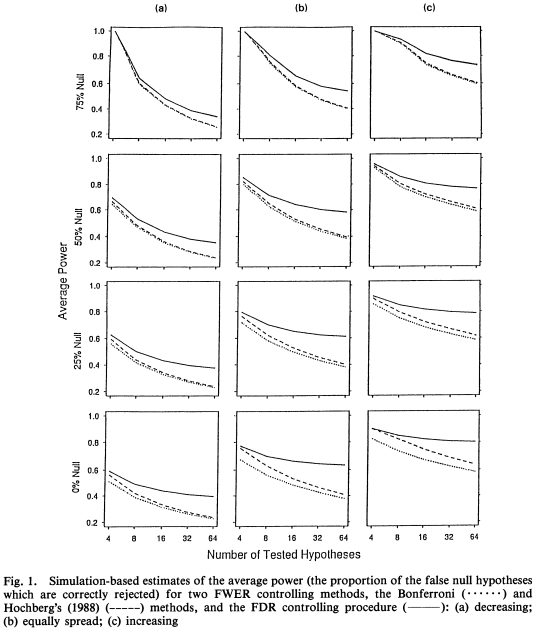
\includegraphics[scale=.7]{figure_1.png}
\end{figure}
\begin{itemize}
\item[(a)] El poder de todos los métodos disminuye cuando aumenta el número de hipótesis probadas; este es el costo del control de multiplicidad. 
\item[(b)] La potencia es más pequeña para la configuración D, donde las hipótesis no nulas están más cerca de la nula, y es más grande para I (lo cual es obvio pero mencionado para completar)
\item[(c)] La potencia del método de control FDR es uniformemente mayor que la de los otros métodos.
\item[(d)] La ventaja aumenta con el número de hipótesis no nulas.
\item[(e)] La ventaja aumenta en m. Por lo tanto, la pérdida de potencia a medida que m aumenta es relativamente pequeña para el método de control FDR en las configuraciones E e I.
\item[(f)] La ventaja en algunas situaciones es extremadamente grande. Por ejemplo, probando 32 hipótesis, igualmente distribuidas en cuatro grupos de 1,25 a 5 para que ninguna sea cierta, el poder del método de Bonferroni es 0,42. El procedimiento sugerido aumenta la potencia a 0,65; probando tan solo cuatro hipótesis, la mitad de las cuales son verdaderas, los valores son 0,62 y 0,70 respectivamente.
\item[(g)] Se sabe que el método de Hochberg ofrece una alternativa más poderosa al método tradicional de Bonferroni. No obstante, es importante señalar que la ganancia de potencia debida al control del FDR en lugar del FWER es mucho mayor que la ganancia del método de control FWER sobre el método de Bonferroni.
\end{itemize}
Al presentar estos resultados en una forma diferente, se puede ver que en algunas configuraciones hasta la mitad de las hipótesis no nulas que no fueron rechazadas por el procedimiento de Bonferroni ahora son rechazadas por el método de control FDR, cuando al menos la mitad de las hipótesis probadas son no nulo. Incluso cuando sólo el $25\%$ de las hipótesis no son nulas, la ganancia de poder es tal que aproximadamente una cuarta parte de las hipótesis igualmente espaciadas que no fueron rechazadas antes ahora se rechazan.\\

La figura 1 nos permite también responder una pregunta planteada por un árbitro, sobre cómo $\mE (V / m_0)$ es controlado por el método de control FDR. Esta tasa de error es 0 cuando $m_0 = 0$ y, de lo contrario, puede aproximarse mediante el nivel medio $\alpha_{ave}$ en el que se prueban las hipótesis individuales. Obviamente, $\alpha_{ave}$ es siempre menor que $q*$, pero para $m_0$ más lejos de $m$ se puede decir más: sea $R_{ave}$ el número promedio de rechazos y $f_{ave}$ sea la potencia promedio (mostrado en la Fig. 1). De ello se deduce que $m\alpha_{ave} <R_{ave} q * = (m\alpha_{ave} + m_1 f_{ave}) q *$, entonces
$$\alpha_{ave}<f_{ave}q*\frac{m_1}{m_1+m_0(1-q*)}.$$
Por lo tanto, $\mE (V / m_0)$ se ve como en la Fig. 1 pero es más pequeño en un factor de $q*$ o incluso menor. Para $m = m_0$, el error está mucho más cerca de $q* / m$, que de $q*: 0.0132, 0.0063, 0.0033, 0.0017$ y 0.0009 para las cuatro, ocho, 16, 32 y 64 hipótesis probadas respectivamente.

\section{CONCLUSIÓN}
El enfoque de las pruebas de significancia múltiple en este artículo es filosóficamente diferente de los enfoques clásicos. El enfoque clásico requiere el control del FWER en el sentido estricto, un control conservador de la tasa de error de tipo I frente a cualquier configuración de las hipótesis probadas. En cambio, el nuevo enfoque exige el control del FDR y, por lo tanto, también el control del FWER en el sentido débil. En muchas aplicaciones, este es el control deseable contra errores originados por multiplicidad.
Dentro del marco sugerido, se pueden desarrollar otros procedimientos, incluidos los procedimientos que utilizan la estructura de problemas específicos, como las comparaciones por pares en el análisis de varianza. Una dirección diferente, que ya hemos seguido, es desarrollar un método adaptativo que incorpore las ideas de Hochberg y Benjamini (1990). En este artículo, sin embargo, solo nos hemos centrado en presentar y motivar el nuevo enfoque que exige controlar el FDR, y hemos demostrado que se puede convertir en un procedimiento simple y poderoso. Por tanto, el coste pagado por el control de la multiplicidad no tiene por qué ser elevado. Esto podría contribuir considerablemente a la proliferación de una mayor conciencia de los problemas de comparación múltiple y de los casos en los que se hace algo al respecto.

\section{AGRADECIMIENTOS}
Nos gustaría expresar nuestro agradecimiento a J.P. Shaffer y J. W. Tukey, cuyos comentarios y preguntas sobre un borrador anterior nos ayudaron a cristalizar el enfoque que aquí se presenta. Agradecemos a Yetty Varon por su participación en la programación del estudio de simulación y a Yechezkel Kling por señalar la necesidad de ajustar la demostración original del teorema 1.

\end{document}